\section{Introduction}
\TODO{This document should contain:}

\subsection{Service overview}

A~fairly complete overview of the \LB service is given in \LB User's Guide~\cite{lbug}.
This section is a~brief excerpt only, providing minimal information necessary for
understanding the rest of this document.

The task of \LB is gathering \emph{\LB events} from various grid middleware components,
and delivering the events to \LB servers where users can query for them.
Figure~\ref{f:gather} shows all principal components involved in the event gathering.

\begin{figure}
\centering
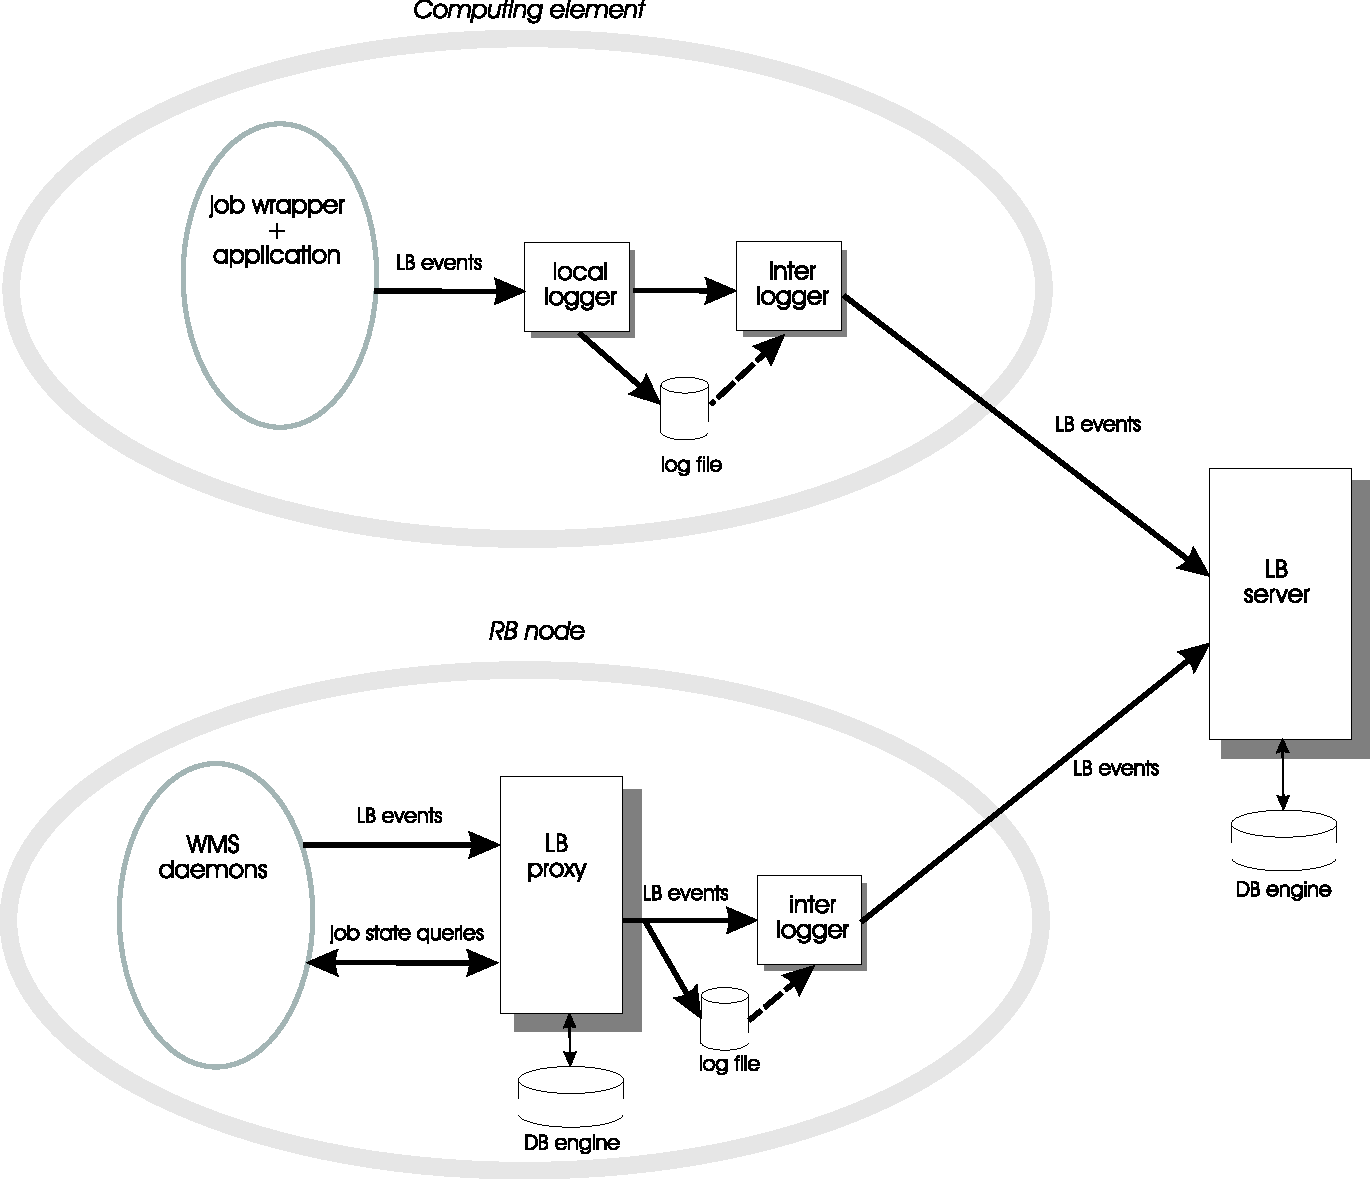
\includegraphics[width=.67\hsize]{LB-components-gather}
\caption{Components involved in gathering and transfering \LB events}
\end{figure}

\begin{figure}
\centering
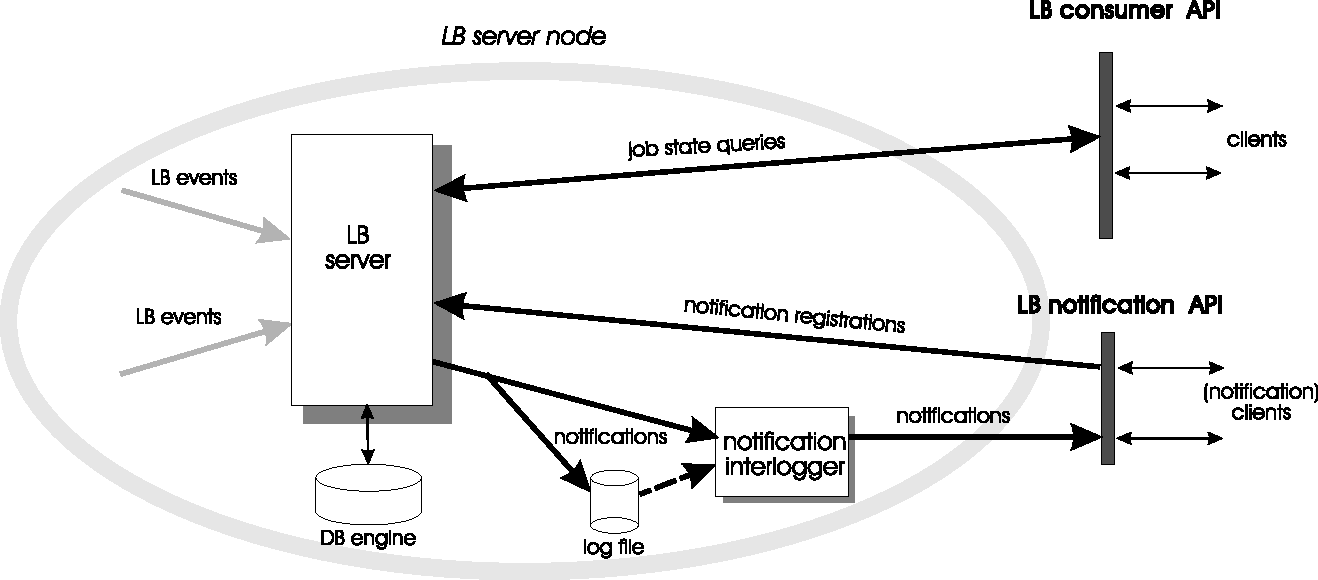
\includegraphics[width=.67\hsize]{LB-components-query}
\caption{\LB queries and notifications}
\end{figure}

\TODO{revize vhodnosti textu wrt. include do AG i UG}
\input components


\subsection{Versions overview}
Mame v tom hokej, verze glite vs. verze LB, co je jak dostupne,
cim se lisi.

Popisovat glite 3.1 a LB 2.0, glite 3.0 prohlasit za obsolete

\subsection{Deployment scenarios}

\TODO{jakou zatez ktery snese}

\subsubsection{Standalone \LB server}

\subsubsection{Hybrid \LB server-proxy}

Jen 2.0

\subsubsection{\LB server on WMS node}
Highly obsolete and inefficient \dots
